\chapter{Background}
\label{chp:background} 

Background from other works:

\section{Remote Attestation}
\label{sec:remote-attestation}

Remote Attestation (RA) always involves a \emph{Prover} and a \emph{Verifier}, 
with the latter responsible for verifying the current status of the former. 
Usually, the \emph{Verifier} sends a challenge to the \emph{Prover} asking to 
measure specific properties. The \emph{Prover}, then, calculates the required 
measurement (\eg a hash of the application loaded) and sends back a report R, 
which contains the measurement M along with a digital fingerprint F, for 
instance, $R = (M,F)$. Finally, the \emph{Verifier} evaluates the report, 
considering its freshness (\ie the report has not been generated through a 
replay attack) and correctness (\ie the \emph{Prover} measurement is valid). It 
is a standard assumption that the \emph{Verifier} is trusted, while the 
\emph{Prover} 
might be compromised. However, the \emph{Prover} is able to generate a correct 
and fresh report due to its trusted anchor (\eg a dedicated hardware module).

\subsection{Runtime RA}

\todo{this is to write entirely}

\section{Control-Flow Attacks}
\label{control-flow-attacks}

To introduce control-flow attacks, we first discuss the concepts of 
control-flow graph~(CFG), execution-path, and basic-block~(BBL) by using the 
simple program shown in Figure~\ref{fig:problem-setting-code} as a reference 
example. 
The program starts with the acquisition of an input from the user (line $1$). 
This is evaluated (line $2$) in order to redirect the execution towards the 
retrieval of a privileged information (line $3$) or an unprivileged one (line 
$4$). Then, the retrieved information is stored in a variable ($y$), which is 
returned as an output (line $5$), before the program properly concludes its 
execution (line $6$). 

\begin{figure}[t]
	\centering
	\begin{subfigure}[t]{0.45\textwidth}
		\centering
		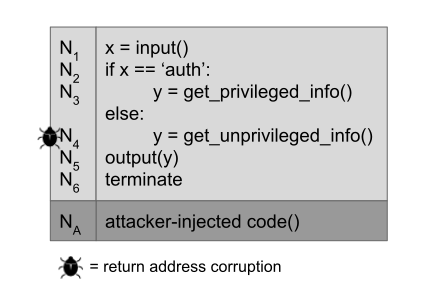
\includegraphics[width=\linewidth]{fig_c4/problem-setting-code.pdf}
		\caption{Pseudo-code of a program under a control-flow attack.}
		\label{fig:problem-setting-code}
	\end{subfigure}
	\hfill
	\begin{subfigure}[t]{0.4\textwidth}
		\centering
		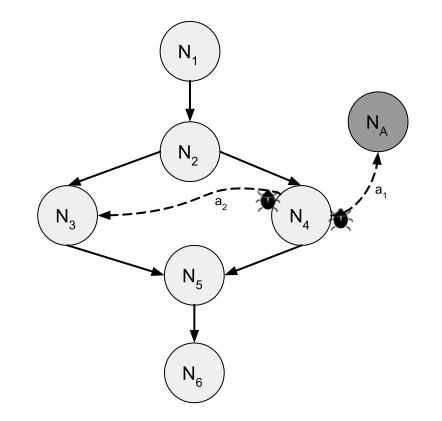
\includegraphics[width=\linewidth]{fig_c4/problem-setting-graph.pdf}
		\caption{Control-flow graph of a program under a control-flow attack.}
		\label{fig:problem-setting-graph}
	\end{subfigure}
	\caption[Example of control-flow attack.]{Illustrative example of a 
	control-flow attack.}
	\label{fig:problem-setting}
\end{figure}

A CFG represents all the paths that a program
may traverse during its execution and it is statically computed. 
On the contrary, an execution path is a single path of the CFG traversed by the 
program at runtime. 
The CFG associated to the program in Figure~\ref{fig:problem-setting-code} is 
depicted in
Figure~\ref{fig:problem-setting-graph} and it encompasses two components: nodes 
and edges. The former are the BBLs of the program, while the latter represent 
the standard flow traversed by the program to move from a BBL towards the next 
one. A BBL is a linear sequence of instructions with a single entry point
(\ie no incoming branches to the set of instructions other than the first), 
and a single exit point (\ie no outgoing branches from the set of instructions 
other than the last). Therefore, a BBL can be considered an atomic unit with 
respect to the control-flow, as it will either be fully executed, or not 
executed at all on a given execution path.
A BBL might end with a control-flow event, which could be one of the following 
in a \texttt{X$86\_64$} architecture: procedure calls (\eg \texttt{call}), 
jumps (\eg \texttt{jmp}), procedure returns (\eg \texttt{ret}), and system 
calls (\eg \texttt{syscall}). 
%Upon certain events (\eg receiving an input), the OS starts a new process.
During its execution, a process traverses several BBLs, which completely define 
the process execution path.

Runtime attacks, and more specifically the control-flow ones, aim at modifying 
the CFG of a program by tampering with its execution path.
Considering Figure~\ref{fig:problem-setting}, we assume that an attacker is 
able to run the program (from the node $N_1$), but that he is not authorized to 
retrieve the privileged information.
However, the attacker can, anyway, violate those controls through a memory 
corruption error performed on the node $N_4$.
As soon as the attacker provides an input to the program and starts its 
execution, he will be redirected to the node $N_4$.
At this point, the attacker can exploit a memory corruption error (\eg a stack 
overflow) to introduce a new edge from $N_4$ to $N_3$ (edge labeled as $a$) and 
retrieve the privileged information.
As a result, the program traverses an unexpected execution path not belonging 
to its original CFG.
Even though several solutions have been proposed to mitigate such attacks (\eg 
ASLR~(\cite{kil2006address})), attackers still manage to perform 
them~(\cite{van2012memory}). 

This illustrative example about how to manipulate the execution path of a 
program is usually the basic step to perform more sophisticated attacks like
exploiting a vulnerability to take control of a 
process~(\cite{yuan2015hardware}) 
or installing a persistent data-only malware without injecting new code, 
once the control over a process is taken by the 
attacker~(\cite{vogl2014persistent}).

%Runtime RA provides a reliable mechanism which allows the \emph{Verifier} to 
%trace and validate the execution path undertaken by the \emph{Prover}. 

\section{Secure Guard eXtension}
\label{sec:secure-guard-extension}

\todo{This comes from the memory forensic paper.}

\subsection{SGX Remote Attestation}

In the SGX Remote Attestation (SGX RA)~\cite{vill2017sgx}, the 
\emph{Prover} is an \emph{enclave}, while the \emph{Verifier} can be either 
another \emph{enclave} or a generic software.
The SGX RA relies on the isolation offered by the CPU to protect the 
cryptographic keys. 
In particular, the SGX RA guarantees two properties:
\begin{enumerate*}[label=(\roman*)]
	\item the host machine has correctly loaded the \emph{Prover} in memory,
	\item the \emph{Verifier} can check the identity of the 
	\emph{Prover} and the machine (\ie CPU) that is loading it.
\end{enumerate*}
However, the SGX RA does not guarantee \emph{runtime} integrity, for instance, 
an adversary can exploit a memory corruption error while the 
\emph{Verifer} cannot detect the attack.

\todo{I could integrate this part with the memory forensic background for the 
CPU structures}

\subsection{SGX Control-Flow Attacks}

In the following, we described the two main works that describe code-reuse 
attacks against SGX: Guard's Dilemma~(\cite{biondo2018guard}) and 
Dark-ROP~(\cite{lee2017hacking}).

\paragraph{Dark-ROP.}
Lee et. al present Dark-ROP~(\cite{lee2017hacking}), a technique to locate 
gadgets in an enclave.
In their scenario, the attacker probes
a victim enclave until triggering an \texttt{AEX}.
From the exception risen, the host can gain information about the location and 
the nature of the gadgets.
Once enough gadgets are collected, the adversary can finally craft a payload 
and bypass the enclave protections.
The success of this technique exploits the fact that neither the enclave 
nor an external observer (\eg the microcode) can backtrack the cause of a 
crash.
In practice, the SGX isolation does not allow inspection either for 
\emph{good} analysis or by adversaries.

\paragraph{Guard's Dilemma.}
Biondo et. al propose a new approach, called \emph{Guard's Dilemma}, that does 
not require probing the enclave~\cite{biondo2018guard}.
The authors abuse two critical Intel SGX SDK procedures to control the CPU 
registers.
The first one is \texttt{asm\_oret}, that restores the CPU registers after an  
OCALL.
The second one is \texttt{continue\_execution}, that is used in the exception
handling.
The authors use the latter to perform a stack pivoting (\ie control the 
\texttt{rsp} register).
\emph{Dilemma} works because the enclave has no mechanism to validate
the integrity of the input of these two functions.

\section{Anti-Tampering Techniques}
\label{anti-tampering-techniques}

We say that a program $P$ is tamper-resistant if $P$ is designed such that an 
attacker would have difficulties to modify $P$'s code.
There are several strategies for achieving this 
goal~(\cite{nagra2009surreptitious}).
In this thesis, we mainly focus on \emph{self-checking}.
These techniques work at bytecode level, and they are structured such that the 
software can read its own bytecode in order to find anomalies and then reacts 
accordingly.
We call \emph{checkers} those sections of the software which check the software 
status, and \emph{responses} those which react to the checkers' requests.

A checker's duties include reading a portion of the software's bytecode and 
verifying whether that code matches specific expectations. That is, the checker 
computes a hash code of the bytecode using a hashing function and compares the 
hash value with a pre-computed value. 
Once a mismatch is found, the software might adopt different reactions, \eg it 
can emit an alarm or restore the un-tampered code. 

To prevent the checkers from being disabled by an attacker, they typically 
spread over the code and/or triggered randomly during the execution.
Checkers, hash functions, and hash values can be prone to attack; therefore, an 
anti-tampering protection must be designed for protecting itself.
This is achievable by using different techniques,
\eg through obfuscation techniques~~\cite{banescu2017tutorial}, or a network of 
checkers (which communicate with each other so that if one checker is 
disabled/tampered, other checkers become aware of the attack).